\chapter{Importing CAD models into a JavaFX window}
\label{chapApp2}

\gls{JPAD} comes equipped with a simple yet very intuitive \gls{acr:GUI}, which provides the user with the possibility to import aircraft data in several ways and perform analyses. Altough the \gls{JPAD} \gls{acr:GUI} currently offers different 2D views of the aircraft (made mostly from the outlines of each of the aircraft components), allowing the user to check the actual configuration and realize quite instantly the changes made to it after modifying some of the available parameters, it would be quite interesting and useful to give also the possibility to view the 3D model of the aircraft, built by means of the \lstinline[language=Java]!JPADCAD! package and the utility functions contained in \lstinline[language=Java]!AircraftUtils!.

\bigskip
\noindent
The Java language offers the possibility to design and create applications such as a simple window for 3D models view and exploration by means of the JavaFX platform \cite{JavaFXPlatform}. JavaFX is a Java library that can be used to build complex applications, that can run consistently across multiple platforms and on various devices, such as desktop computers, mobile phones, TVs, tablets, etc. In general, a JavaFX application has three major components, namely \emph{Stage}, \emph{Scene}, and \emph{Nodes}. The stage (a window) contains all the objects of a JavaFX application, and is represented by the \lstinline[language=Java]!Stage! class. The primary stage is automatically created by the platform itself and is passed as an argument to the \lstinline[language=Java]!start! method of the \lstinline[language=Java]!Application! class, the abstract class from which all the JavaFX applications extend. A scene, instead, represents the physical contents of a JavaFX application. It contains the \emph{Scene Graph}, which is a tree-like data structure, whose root, branches, and leaves are represented by nodes. A node, in general, may include:
%
\begin{itemize}
\item geometrical objects, such as circles, rectangles, polygons, etc.;
\item controls, such as buttons, check box, choice box, text area, etc.;
\item containers, such as border pane, grid pane, flow pane, etc.;
\item media elements, such as audio, video, and image objects.
\end{itemize}
%
A branch node (also called parent node) is a node with child nodes. There are several types of parent nodes, the most used of which is the \emph{Group} one. A group node is a collective node and whenever the group node is rendered, all its child nodes are rendered in order. Any transformation applied on the group is applied to all the child nodes.

\bigskip
\noindent
The objects that we want to import into a JavaFX window are much more complicated than the ones that can be created by using the three built-in 3D shape classes that come with JavaFX: \lstinline[language=Java]!Cylinder!, \lstinline[language=Java]!Box!, and \lstinline[language=Java]!Sphere!. For more complex objects, the JavaFX library provides the user with the \lstinline[language=Java]!TriangleMesh! class, which allows to create objects based on a connected series of triangles. In order to create the necessary \lstinline[language=Java]!TriangleMesh! objects, which should represent the 3D shapes of the aircraft obtained by the use of \lstinline[language=Java]!JPADCAD!, it is crucial some sort of conversion from \lstinline[language=Java]!TopoDS_Shape! (the generic \gls{OCCT} class managing all sort of shapes) to \lstinline[language=Java]!TriangleMesh! entities. \lstinline[language=Java]!OCCDataProvider! and \lstinline[language=Java]!OCCFXMeshExtractor! are the \lstinline[language=Java]!JPADCAD! classes providing the instruments for this operation. In particular, to generate a \lstinline[language=Java]!TriangleMesh! instance three collections must be defined: one for the points, one for the faces, and one for the texture coordinates. The \lstinline[language=Java]!OCCFXMeshExtractor! class, along with its \lstinline[language=Java]!FaceData! sub-class (which extends the generic \lstinline[language=Java]!OCCDataProvider! one), allows to automatically convert \lstinline[language=Java]!TopoDS_Face! objects to \lstinline[language=Java]!TriangleMesh! entities, by employing the face object underlying mesh data structure (handled by the \gls{OCCT} \lstinline[language=Java]!BRepMesh_IncrementalMesh! class). In this way, the aircraft 3D model (its face-type shapes) can be converted into a list of sub-lists of \lstinline[language=Java]!TriangleMesh! entities, with each sub-list being relative to a particular aircraft component (listing \ref{lst:FaceConversion}).
%
\bigskip
\begin{lstlisting}[caption={Solid shapes conversion to JavaFX triangle meshes}, captionpos=b, tabsize=2, label={lst:FaceConversion}]
// Import the aircraft into the application
Aircraft theAircraft = AircraftUtils.importAircraft(args);

// Generate selected aircraft solid shapes
List<ComponentEnum> comps = new ArrayList<>();
comps = Arrays.asList(new ComponentEnum[] {
		ComponentEnum.FUSELAGE, 
		ComponentEnum.WING, 
		ComponentEnum.HORIZONTAL_TAIL, 
		ComponentEnum.VERTICAL_TAIL, 
		ComponentEnum.CANARD
});

List<OCCShape> allShapes = AircraftUtils.getAircraftShapes(theAircraft, comps);
List<TopoDS_Solid> solids = AircraftUtils.getAircraftSolid(allShapes);
		
// Extract the triangle meshes
List<List<TriangleMesh>> triangleMeshes = solids.stream()
	.map(s -> (new OCCFXMeshExtractor(s)).getFaces().stream()
		.map(f -> {
			FaceData faceData = new FaceData(f, true);
			faceData.load();
			return faceData.getTriangleMesh();
		})
		.collect(Collectors.toList()))
	.collect(Collectors.toList());
\end{lstlisting}
%

\bigskip
\noindent
The converted faces are then added to a group, after being given a specific color based on the aircraft surface they belong to. This group, in turn, is added to another one, which acts as a camera for the final scene. The result is shown in the following figure, which depicts four different aircrafts imported into a JavaFX window by the means of the same application. The next step, obviously, will consist in adding the so-created window to the \gls{JPAD} \gls{acr:GUI}.
%
\begin{figure}[H]
\centering
\includegraphics[scale=0.51]{Immagini/Appendice/javafx_01}
\caption{\lstinline[language=Java]!JPADCAD! aircrafts imported into the JavaFX application}
\label{fig:javafx_01}
\end{figure}
% 